%--------------------------------------------------------------------
%--------------------------------------------------------------------
% Formato para los talleres del curso de Métodos Computacionales
% Universidad de los Andes
%--------------------------------------------------------------------
%--------------------------------------------------------------------

\documentclass[11pt,letterpaper]{exam}
\usepackage[utf8]{inputenc}
\usepackage[spanish]{babel}
\usepackage{graphicx}
\usepackage{tabularx}
\usepackage[absolute]{textpos} % Para poner una imagen en posiciones arbitrarias
\usepackage{multirow}
\usepackage{float}
\usepackage{hyperref}
%\decimalpoint

\begin{document}
\begin{center}
{\Large Métodos Computacionales} \\
\textsc{Tarea 2}\\
01-2019\\
\end{center}

\noindent
\section{Ejercicio 1: Fourier}
\subsection{subplots de senales sumadas e individuales} 
\begin{center}
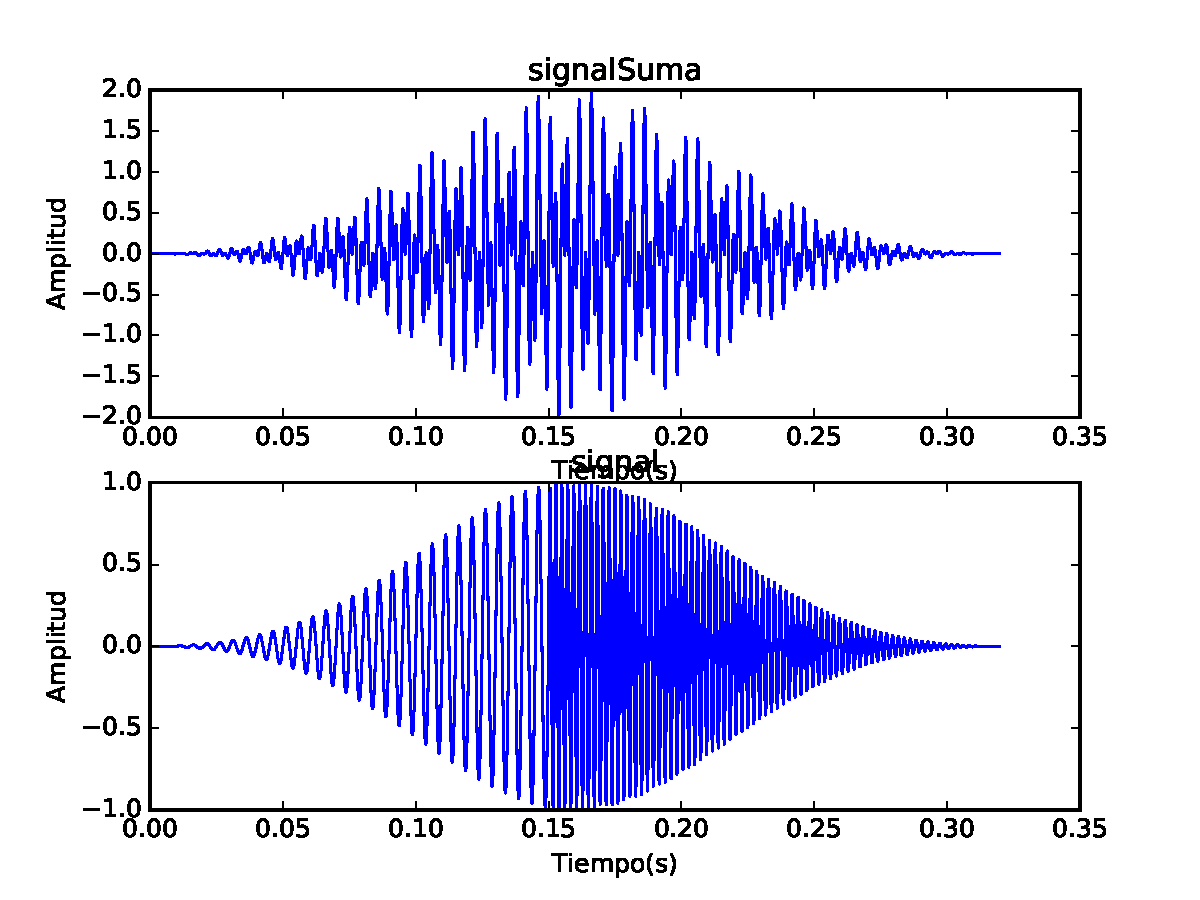
\includegraphics[width=10cm]{signal_subplots.pdf} 
\end{center}
En este grafico vemos representadas las senales sumadas en el plot superior y las individuales en el inferior. Se puede ver como varia la amplitud y la frecuencia, para el caso inferior, en el tiempo.

\subsection{Transormada de Fourier para las senales}
\begin{center}
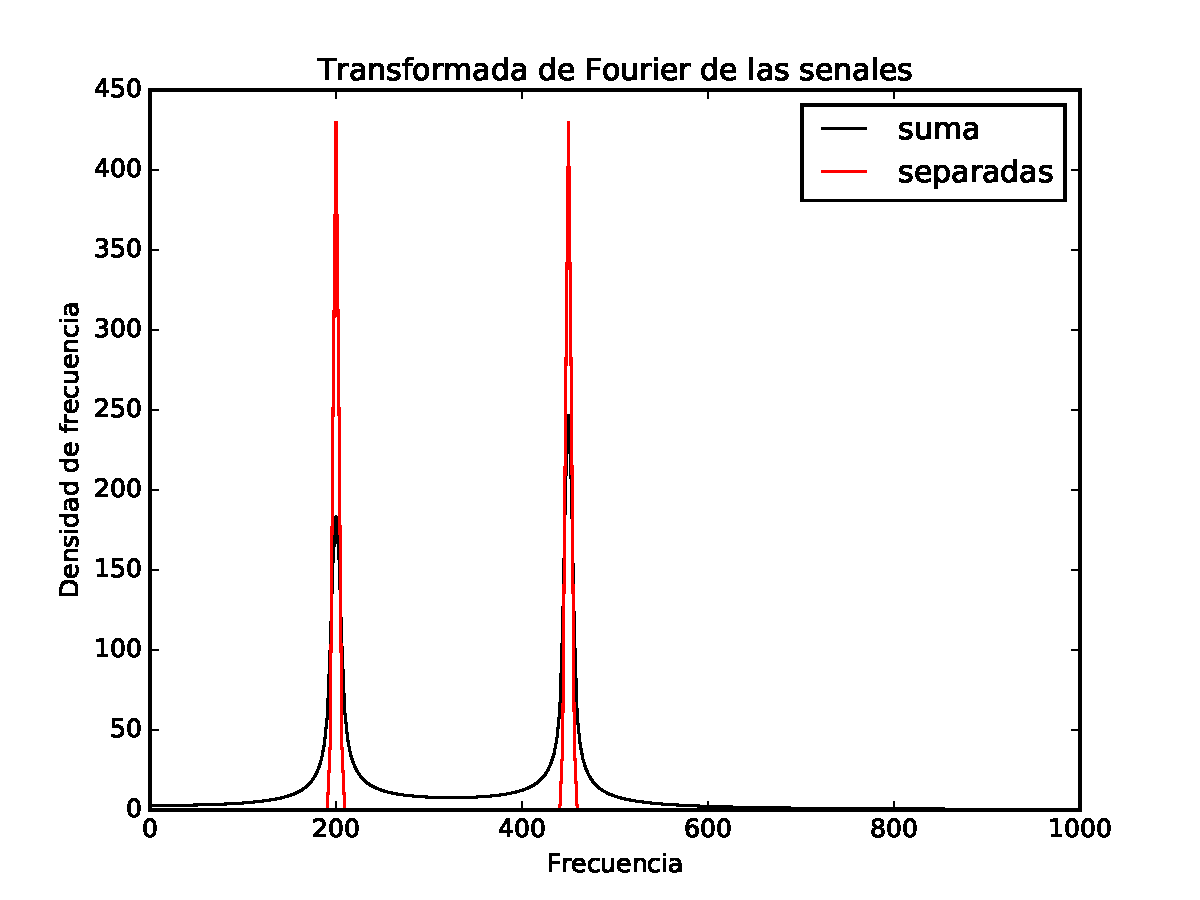
\includegraphics[width=10cm]{Fourier_senales.pdf} 
\end{center}
El grafico muestra la transformada de Fourier para ambas senales. Como se esperaba hay dos picos que indican los modos normales de cada senal, vemos que los picos de la suma son significativamente menores que los de las senales individuales.

\subsection{Espectrograma para las senales}
\begin{center}
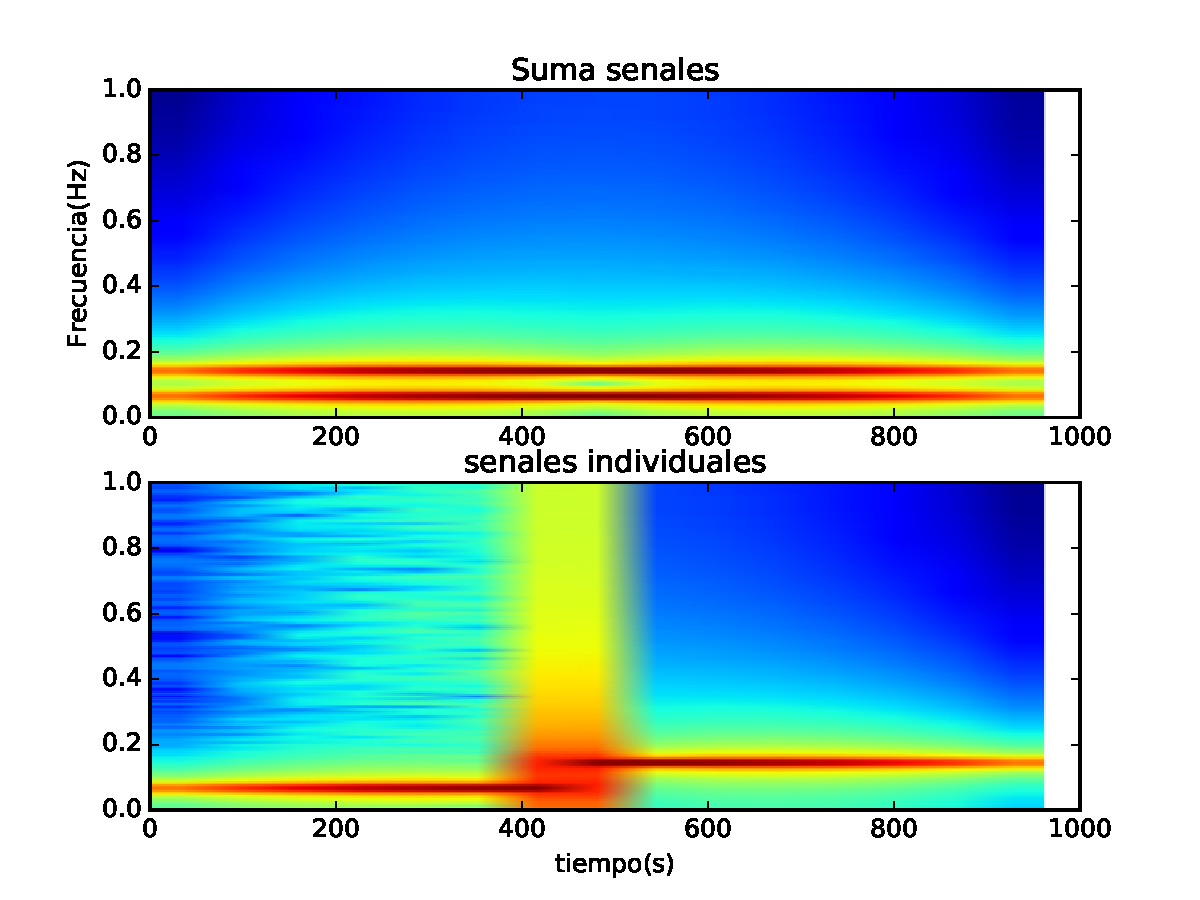
\includegraphics[width=10cm]{espectrogramas1.pdf} 
\end{center}
Los espectrogramas de las senales nos permiten visualizar mejor como estas se comportan, ya que en un grafico de 3 dimensiones podemos ver como la amplitud y la frecuencia se comportan en funcion del tiempo. En el grafico los colores rojos indican las mayores amplitudes, mientras que los azules/aguamarina indican las amplitudes mas pequeñas. Podemos ver que en el eje Y tenemos las frecuencias, por lo que vemos las lineas rojas paralelas al eje X indicando las frecuencias de los modos normales de estas senales. En el subplot de las senales individuales vemos una franja amarilla centrada, indicando el momento donde pasamos de la lectura de una senal a otra.

\subsection{Senal de un temblor real}
\begin{center}
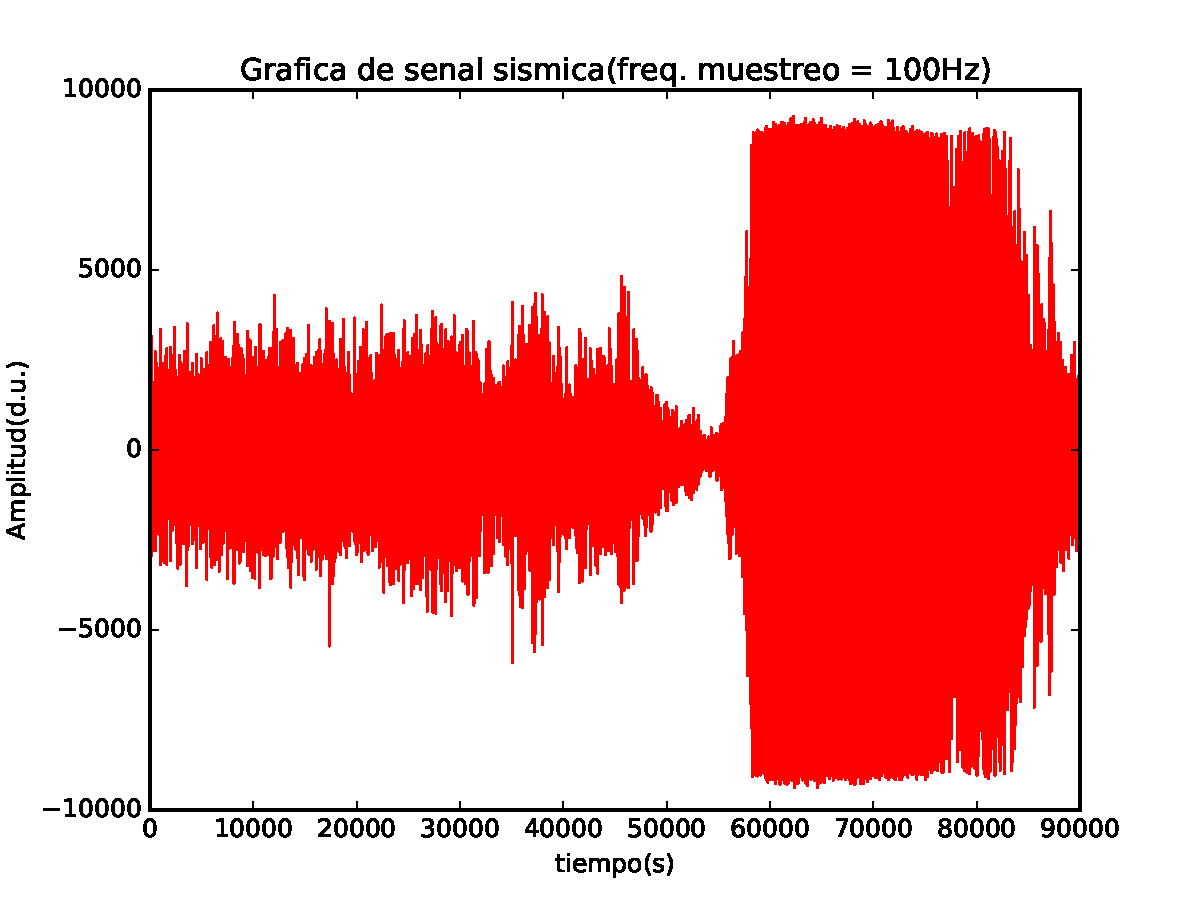
\includegraphics[width=10cm]{temblor.pdf} 
\end{center}
Este grafico es un sismograma de una senal de temblor real, podemos ver como comienza con una amplitud constante natural, posteriormente vemos como hay una disminucion de esta amplitud seguida de un drastico incremento de esta, lo que representa el comienzo del temblor.

\subsection{Transformada de Fourier senal de temblor}
\begin{center}
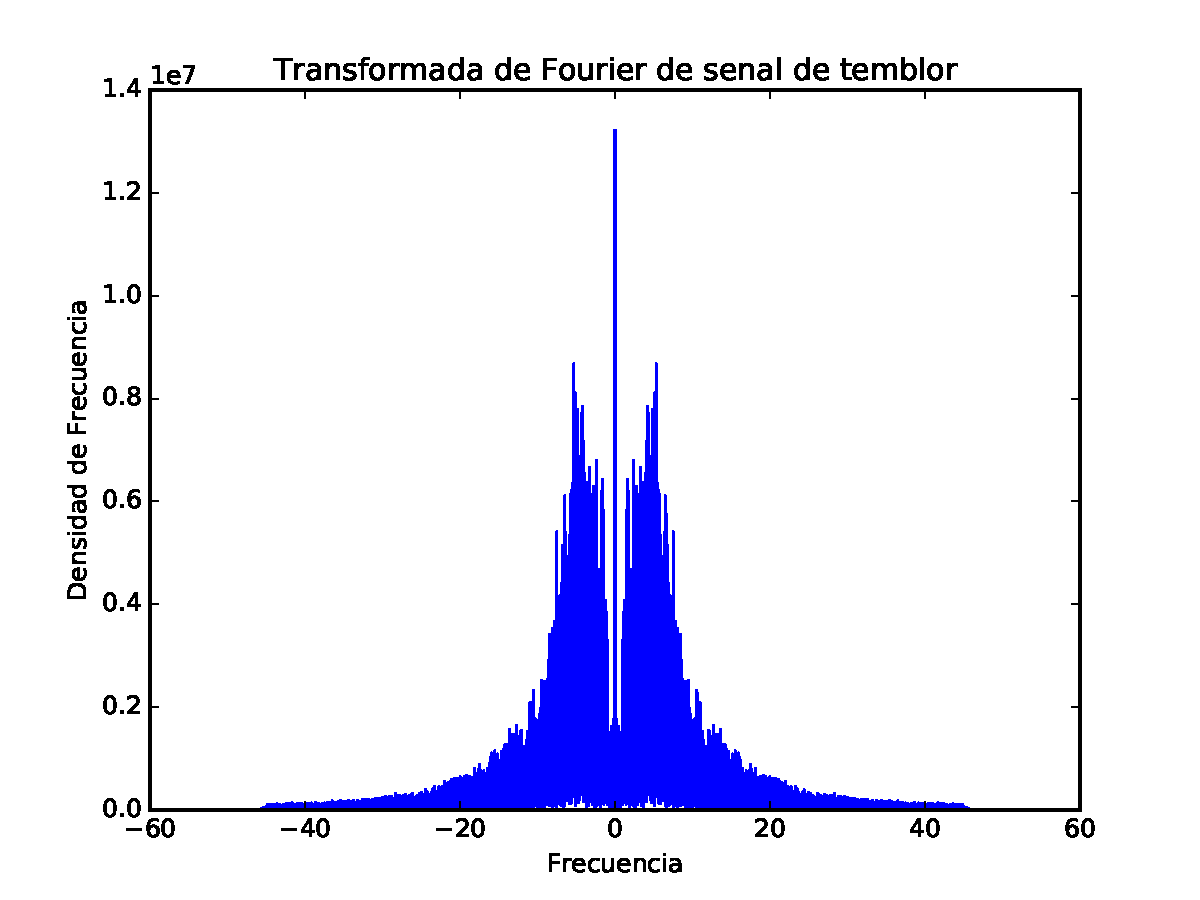
\includegraphics[width=10cm]{Fourier_temblor.pdf} 
\end{center}
La transformada de Fourier de la senal permite pasar al espacio de frecuencia representado en este grafico. En el grafico vemos que hay un pico alrededor de una frecuencia de 10Hz indicando el modo normal de esta senal.

%Analisis de resultados...

\end{document}
